\section{Dipole Calculus Family}\label{sec:dipole}

A dipole is an oriented line segment as e.g.\ determined by a start and an end point. We will write $\vec{d}_{AB}$ for a dipole defined by start point $A$ and end point $B$.
The idea of using dipoles was first introduced by \citet{schlieder95_reasoning} and extended resulting in the coarse-grained Dipole Relation Algebra \DRAc{} \citep{moratz-renz-wolter-ECAI:00}. Later,
a fine-grained version of the dipole calculus ($\mathcal{DRA}_{f}$) has
been proposed \citep{cosy:dylla:2004:qsnhinsitcalc_b} and which has further been extended to $\mathcal{DRA}_{fp}$ \citep{cosy:dylla:2004:qsnhinsitcalc_b}.
In \engine{}, currently only the coarse-grained version \DRAc{} is available.


\subsection*{Coarse-grained Dipole Relation Algebra (\DRAc)}\label{sec:dipole-coarse}

\kasten{
\subsubsection*{Coarse-grained dipole calculus (\DRAc) overview}
\begin{calcfeatures}
\feature{calculus identifier}{dra-24, dipole-coarse}
\feature{calculus parameters}{none}
\feature{arity}{binary}
\feature{entity type}{dipoles in the plane (oriented line segments)}
\feature{description}{relates two dipoles using the FlipFlop relations
between the start and end point of one dipole and the other dipole}
\feature{base relations}{4-symbol words where each symbol can
be either l (left), r (right), s (start), or e (end) (not all combinations are possible)}
\lastfeature{references}{\citet{moratz-renz-wolter-ECAI:00}}
%\feature{remarks]
\end{calcfeatures}
}
\begin{figure}[ht]
 	\centering
% 	\includegraphics[width=0.4\textwidth]{DRAf_rlll+_Example}
	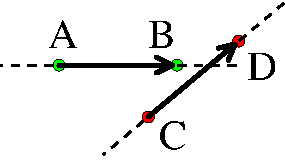
\includegraphics[width=0.3\textwidth]{dra-ex}
	\caption{A dipole configuration: $\vec{d}_{AB}~rlll~\vec{d}_{CD}$ in the coarse-grained dipole relation algebra ($\mathcal{DRA}_{c}$).}
	\label{fig:DRAf}
\end{figure}

The coarse-grained dipole calculus variant ($\mathcal{DRA}_{c}$) describes the orientation relation between two dipoles $\vec{d}_{AB}$ and  $\vec{d}_{CD}$ with the preliminary of $A$, $B$, $C$, and $D$ being in general position, i.e.\ no three disjoint points are collinear.
Each base relation is a 4-tuple $(r_1,r_2,r_3,r_4)$ of FlipFlop relations
relating a point from one of the dipoles with the other dipole.
$r_1$ describes the relation of $C$ with respect to the dipole  $\vec{d}_{AB}$, $r_2$ of $D$ with respect to  $\vec{d}_{AB}$, $r_3$ of $A$ with respect to $\vec{d}_{CD}$, and $r_4$ of $B$ with respect to $\vec{d}_{CD}$. The distinguished
FlipFlop relations are \textbf{l}eft, \textbf{r}ight, \textbf{s}tart,
and \textbf{e}nd (see Fig.~\ref{fig:FFC}). Dipole relations are usually written without commas and parentheses, e.g. $rrll$. Thus, the example in Fig.~\ref{fig:DRAf} shows the relation $\vec{d}_{AB}~rlll~\vec{d}_{CD}$.
Since the underlying points for a $\mathcal{DRA}_{c}$ relation need to be in
general position, $r_i$ can only take the values \textbf{l}eft, \textbf{r}ight, \textbf{s}tart, or \textbf{e}nd resulting in 24 base relations.


%\subsection*{fine grained dipole ($\mathcal{DRA}_{f}$)}
%
%A dipole is an oriented line segment as e.g. determined by a start and an end point. We will write $\vec{d}_{AB}$ for a dipole defined by start point $A$ and end point $B$. The fine-grained dipole calculus ($\mathcal{DRA}_{f}$) \ref{cosy:dylla:2004:qsnhinsitcalc_b} describes the orientation relation between two dipoles $\vec{d}_{AB}$ and  $\vec{d}_{CD}$. Each base relations is 4-tuple $(r_1,r_2,r_3,r_4)$ of FlipFlop relations. $r_1$ describes the relation of $C$ with respect to the dipole  $\vec{d}_{AB}$, $r_2$ of $D$ with respect to  $\vec{d}_{AB}$, $r_3$ of $A$ with respect to $\vec{d}_{CD}$, and $r_4$ of $b$ with respect to $\vec{d}_{CD}$. The relations are usually written without the commas, e.g. (rrll). Thus, the example in figure \ref{fig:DRAfp} s shows the relation $\vec{d}_{AB}$ (rlll) $\vec{d}_{CD}$. $\mathcal{DRA}_{f}$ has 72 base relations.
%
%\begin{figure}[htp]
%	\centering
%	\includegraphics[width=0.5\textwidth]{pics/DRAf_rlll+_Example}
%	\caption{A dipole configuration: $\vec{d}_{AB}$ (rlll) $\vec{d}_{CD}$ in the fine-grained dipole relation algebra ($\mathcal{DRA}_{f}$) or  $\vec{d}_{AB}$ (rlll+) $\vec{d}_{CD}$ in the extended version $\mathcal{DRA}_{fp}$.}
%	\label{fig:DRAfp}
%\end{figure}

% An extended version called $\mathcal{DRA}_{fp}$ \ref{cosy:dylla:2004:qsnhinsitcalc_b} further classifies the angle $s$  that would result from translating $\vec{d}_{CD}$ so that both start points coincide. Four cases are distinguished: \textbf{P}arallel ($s=0^\circ$), \textbf{A}ntiparallel ($s=180^\circ$), \textbf{+} ($s\in]0^\circ..180^\circ[$), and \textbf{-} ($s\in]180^\circ..360^\circ[$). This results in 80 base relations and the example from figure \ref{fig:DRAfp} depicts the  $\mathcal{DRA}_{fp}$ relation (rlll+).

%\subsection*{?}
